\documentclass[times, 10pt,twocolumn]{article} 
\usepackage{latex8}
\usepackage[utf8]{inputenc}
\usepackage{times}
\usepackage{graphicx}
\usepackage[font=small,labelfont=bf]{caption}
\pagestyle{empty}

%------------------------------------------------------------------------- 
\begin{document}


\title{HillClimb@Cloud \\ Cloud Computing and Virtualization \\MEIC-IST }

\author{83531 -Miguel Belém - miguelbelem@tecnico.ulisboa.pt\\
83567 - Tiago Gonçalves - tiago.miguel.c.g@tecnico.ulisboa.pt\\
83576 - Vítor Nunes - vitor.sobrinho.nunes@tecnico.ulisboa.pt
}

\maketitle
\thispagestyle{empty}

\begin{abstract}
   This paper talks about the first phase of a project that makes usage of
   code instrumentation to obtain metrics to create a Load Balancer and 
   Auto Scaler for a Cloud Based Solution.
\end{abstract}

\Section{Introduction}
   This project consists on developing a Load Balancer and Auto-Scaler for 
   a program running on Amazon Web Services that searches for the maximum value 
   of a map using different search strategies (A*, BFS, DFS). For that, we instrumented
   the code so we could produce metrics about the running instances and adapt the system 
   to get the maximum value of the instances running in AWS at a minimum cost.\\
   Although this project uses a specific program to load the instances its objective 
   is to be able to generalize the procedure in a way that the Load balancer and 
   auto scaler would work even if the given program is completely different.

%-------------------------------------------------------------------------

\Section{Architecture}
   For this checkpoint we have AWS running instances of a WebServer which 
   receives the requests from the client. To manage the load we made use of
   a classic Load Balancer of Amazon Web Services along with a Auto Scaling Group 
   to manage the running instances and to allow a scale mechanism while we don't 
   implement our own Load Balancer and Auto Scaler for next phase of the project.

%-------------------------------------------------------------------------
\SubSection{Template Instance}
   We created a Linux instance based on the Linux AMI AWS - t2.micro image, 
   which is the one eligible for free tier usage on AWS. It has a single core
   (up to 3.3 Ghz) and 1 GB of RAM. The Linux distribution was updated and
   extra packages needed for running the WebServer and BIT were installed.
   We loaded the Web Server that takes the requests to the instance and 
   altered on-boot scripts to start up the Web Server every time that
   the system is booted.\\
   We created an AMI so that we could replicate the instance and use it 
   on a Load Balancer and Auto Scaling Group.

%-------------------------------------------------------------------------
\SubSection{Load Balancer}
   We created a Classic Load Balancer on AWS. The Load Balancer receives HTTP
   requests on its port 80 and redirects it to the instances also using HTTP
   protocol but on port 8000. For the security group we allowed every communication
   coming to port 22 that uses SSH protocol (to allow remote access) and every
   message that uses HTTP to port 80 and 8000. The instances verification is made 
   by pinging in a 30 seconds interval the Web Server running in the instances 
   using HTTP protocol on the port 8000. An instance is flagged as unhealthy after
   2 failed pings from the LB and deemed as healthy if pinged successfully 10 consecutive 
   times.\\
   To fulfill the ping requests we modified the Web Server to answer to null queries
   so the LB can simply make an HTTP to http://instanceip/climb.
   
%-------------------------------------------------------------------------
\SubSection{Auto Scaling Group}
   We created an Auto Scaling Group on AWS that increases the number of instances by
   1 if the average CPU utilization is over 60 \% in a period of 5 minutes and
   decreases the number of instances by 1 (to a minimum of 1 instance) if the average CPU 
   utilization of all instances is under 40\% for a period of 5 minutes. This allows
   to scale up in a situation of continuous heavy load while not scaling down instantly
   if we get a slight pause of incoming requests. \\
   We want to be careful shuting down instances as they take some time starting up and if 
   we get a temporary decrease and terminate them and then we might get back to a state
   where we can't deal with all requests that turns to a higher response time to those 
   requests. To avoid this we wait to see if the decrease of requests (lower CPU usage)
   is not temporary (hence the 5 minutes under 40\% CPU load). Also if for some reason
   an instance becomes unhealthy (unresponsive or the WebServer crashed for some reason)
   then the auto-scaler will terminate that instance and start another.

\SubSection{Security Group}

%------------------------------------------------------------------------- 
\Section{Instrumentation}
   We used BIT (Bytecode Instrumenting Tool) presented in the laboratories to 
   to alter the Java Class Byte Code of the program so we could measure the metrics
   that we wanted in a way that would help us decide the cost of replying to a certain request.\\
   This metrics need to be heavily weighted as they might give a big overhead to the 
   the original program. To store this metrics we created a class called Metrics, which
   stores all of the counter for each type of metric. We guarantee that each thread only 
   counts its own metrics by using a ConcurrentHashMap to store all the metrics, where the 
   key is the Thread ID and the Value is the Metrics Object (containing all the metrics). At 
   the end of each request we store permanently the results of the instrumentation and remove
   the Metrics file from the HashMap, this allows to reset the counters for that specific thread.\\
   With the metrics it's also stored the parameters given to program so we can associate those with
   the load it creates and in the future compare them with new requests.


%-------------------------------------------------------------------------    
\SubSection{Metrics Used}
   We decided to try a few simple metrics. Instructions run, Basic Blocks, 
   Methods Called, Branches Queries, Branches Taken and Branches not taken. 
   We ran the instrumented Web Server on an instance of AWS and made some requests 
   (one at a time) while tracking the time it took to reply to each request.
   We obtained a table with all the values and concluded that some metrics grew
   linearly with the time to reply a request. Those metrics were Instructions
   Run, Basic Blocks, Branches and Branch not Taken.\\
   Methods Called and Branch Taken were inconsistent because they depended on 
   the search algorithm being used and do not necessarily mean a higher cost to 
   reply to a request as different methods could have different number of instructions
   which could mislead the cost of the request.\\
   As the other metrics scaled linearly with the time to reply to the request we can
   associate a higher number on this metrics to a more CPU intensive task.
   We decided to stick with Basic Blocks and Branches not Taken due to its 
   linear grow matched with response time to the request and also because they provided
   the lower overhead to the running code. 

%-------------------------------------------------------------------------
\SubSection{Storing the metrics}
   After each request we are storing the Metrics object on a binary file locally
   to the machine and we also add those metrics to a table on Dynamo-DB.
   Each request has its own file with its metrics and it's named by its by 
   a sequence id local to the instance.\\
   To later access this binary file we also create a Java Class, LogReader, 
   which reads the metrics binary files and prints those values so that we can 
   use the values in next stage to calculate the cost of a request to
   system.

%------------------------------------------------------------------------- 

\Section{Future Work}
\SubSection{Metrics}
   At this point of the project the Web Server at the end of every request 
   it writes the metrics to a local (to the instance) binary file and it 
   also writes them to a table on Dynamo-DB. At this time we don't have 
   a common key between all instances (we're using the Thread ID), eventually
   a metric that is on the table will be overwritten by another metric, which 
   we don't want. With this in the next phase we should design a synchronized
   identifier to use with all instances metrics.


\SubSection{Load Balancer}
   We will stop using AWS LB and will create a special instance to run as the 
   Load Balancer that will use the metrics generated by the Worker Servers to
   decide the cost of a request and to which Worker should the new request be
   sent to. We will compare new requests with old requests that we already ran
   and will try to match them to find out the cost of the new one and decide
   the better instance to run it.\\ 
   The Load Balancer will also send information to the new Auto Scaler so it 
   can make decisions on the number of instances that should be running.

\SubSection{Auto Scaler}
   Just as the LB we will stop using the default AWS Auto Scaler and create our 
   own auto scaler on a special instance to manage the running instances that will 
   receive feedback from the LB and depending of the state of the system it will
   increase or decrease the number of instances running.\\\\

%-------------------------------------------------------------------------
\Section{Appendix - Metrics Measurements}
\begin{figure}[!htb]
   \centering
   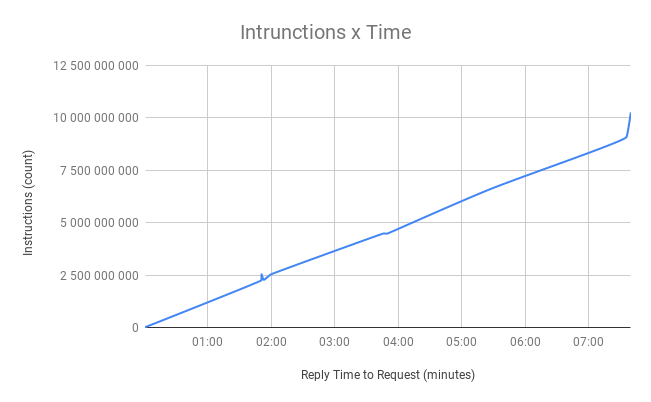
\includegraphics[width=\columnwidth]{images/Intrunctions.png}
   \caption{}
\end{figure}
\begin{figure}[!htb]
   \centering
   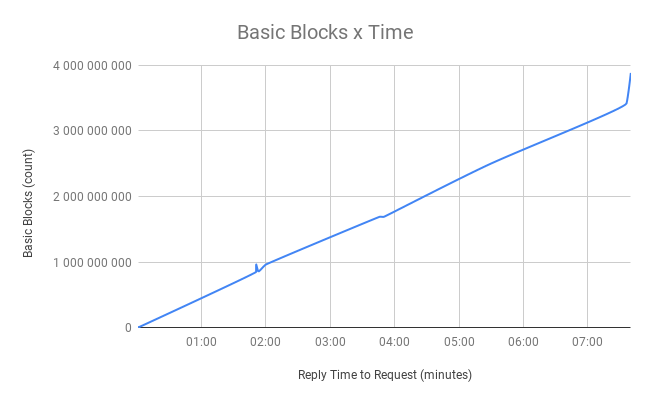
\includegraphics[width=\columnwidth]{images/BB.png}
   \caption{}
\end{figure}
\begin{figure}[!htb]
   \centering
   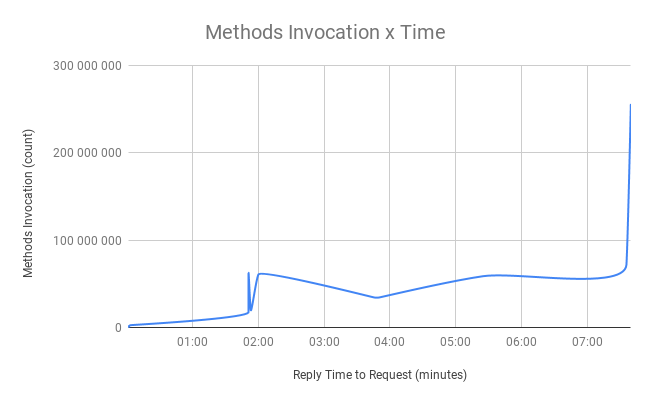
\includegraphics[width=\columnwidth]{images/Methods.png}
   \caption{}
\end{figure}
\begin{figure}[!htb]
   \centering
   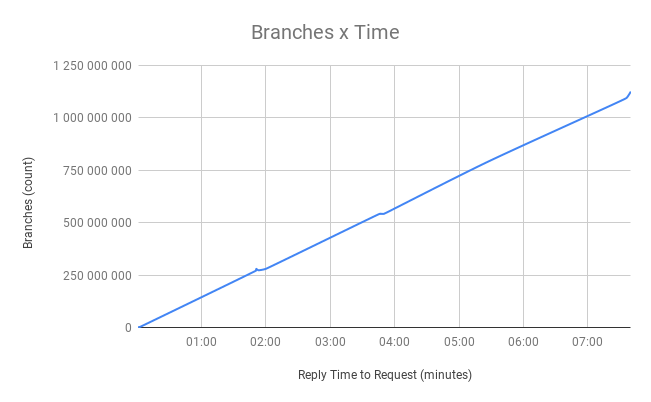
\includegraphics[width=\columnwidth]{images/Branches.png}
   \caption{}
\end{figure}
\begin{figure}[!htb]
   \centering
   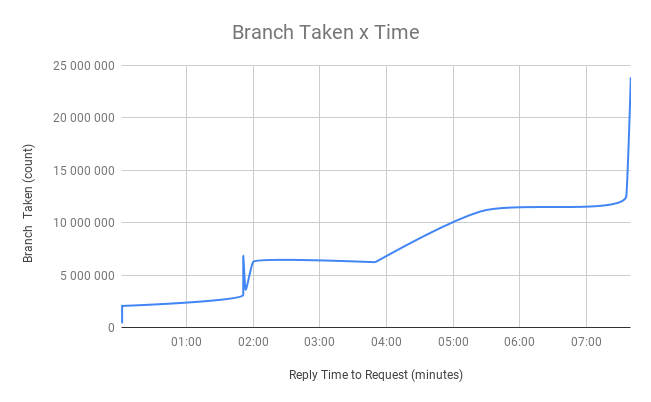
\includegraphics[width=\columnwidth]{images/Taken.png}
   \caption{}
\end{figure}
\begin{figure}[!htb]
   \centering
   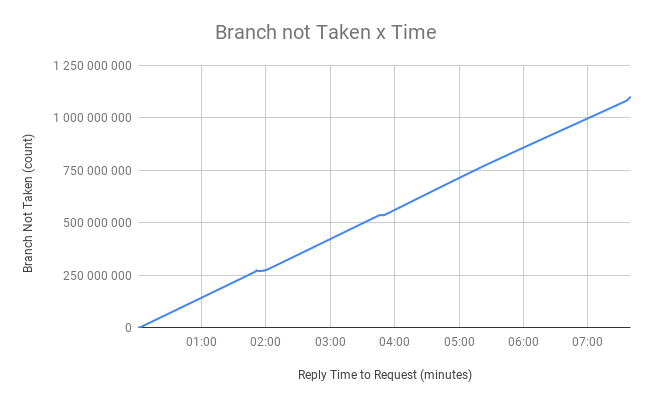
\includegraphics[width=\columnwidth]{images/NotTaken.png}
   \caption{}
\end{figure}

\end{document}

